%------------------------------------------------
% 		LEVEL 1
%------------------------------------------------
\subsection*{Level 1}
\addcontentsline{toc}{subsection}{Level 1}

The embedded Matlab implementation leads to the exact same result than the implementation using ordinary Simulink blocks. Indeed, since we use a discretized controller, transposing the simulink code to the embedded Matlab implementation produces a code with the same behavior as the one produced by Simulink.

Figure \ref{embedded} shows the superposition of the embedded implementation and the one using Simulink.

See Appendix \ref{appendixCode} for the Matlab code.

\begin{figure}[ht]
  \centering
  \begin{subfigure}[b]{\linewidth}
   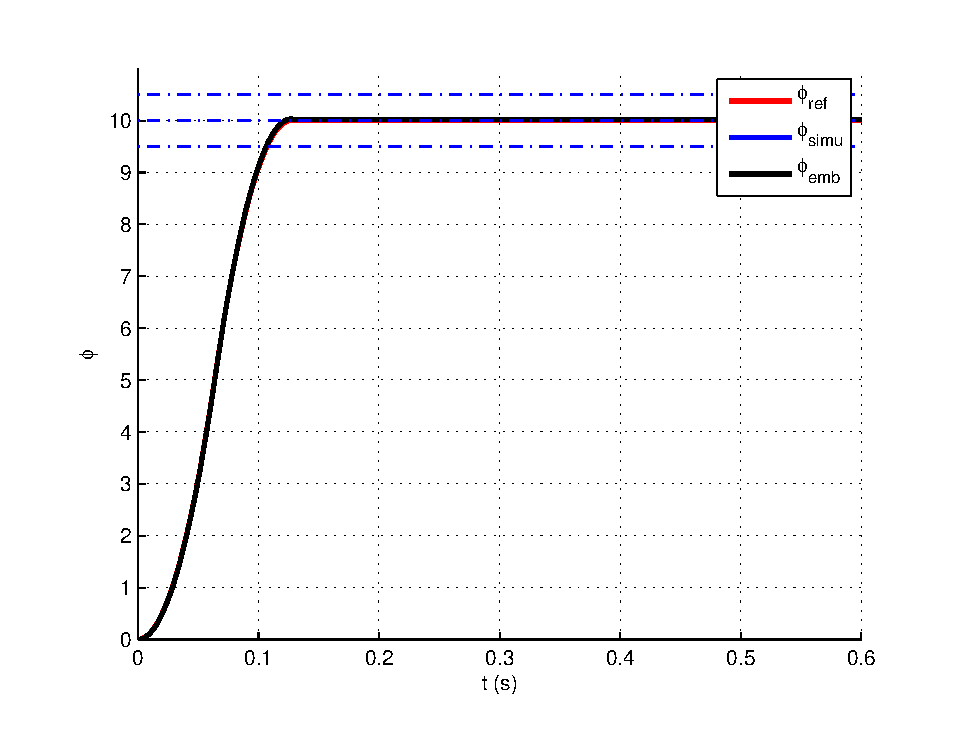
\includegraphics[width=\columnwidth]{fig/embeddedlvl110.eps}
   \caption{$Rs = 10$[rad]}
  \end{subfigure}
  \begin{subfigure}[b]{\linewidth}
  \includegraphics[width=\columnwidth]{fig/embeddedlvl1100.eps}
   \caption{$Rs = 100$[rad]}
  \end{subfigure}

 \caption{Result with a embedded controller}
 \label{embedded}
\end{figure}

%------------------------------------------------
% 		LEVEL 2
%------------------------------------------------
\subsection*{Level 2}
\addcontentsline{toc}{subsection}{Level 2}

Once we had the model following controller with both Simulink and embedded Matlab implementmation, we ran it on the real motor. Figure \ref{realresults} shows the two step responses, using the two differents methods. As previously, the two curves are almost alentirely merged.

Moreover, since our controller is designed in such a way that the motor is accelerating at $0.75 a_{max}$ and moving at most at a velocity of $0.75 v_{max}$, the trajectory planner provide safe trajectories. The step response are therefore almost the same as the one simulated.

\begin{figure}[hb]
  \centering
 \begin{subfigure}[b]{\linewidth}
 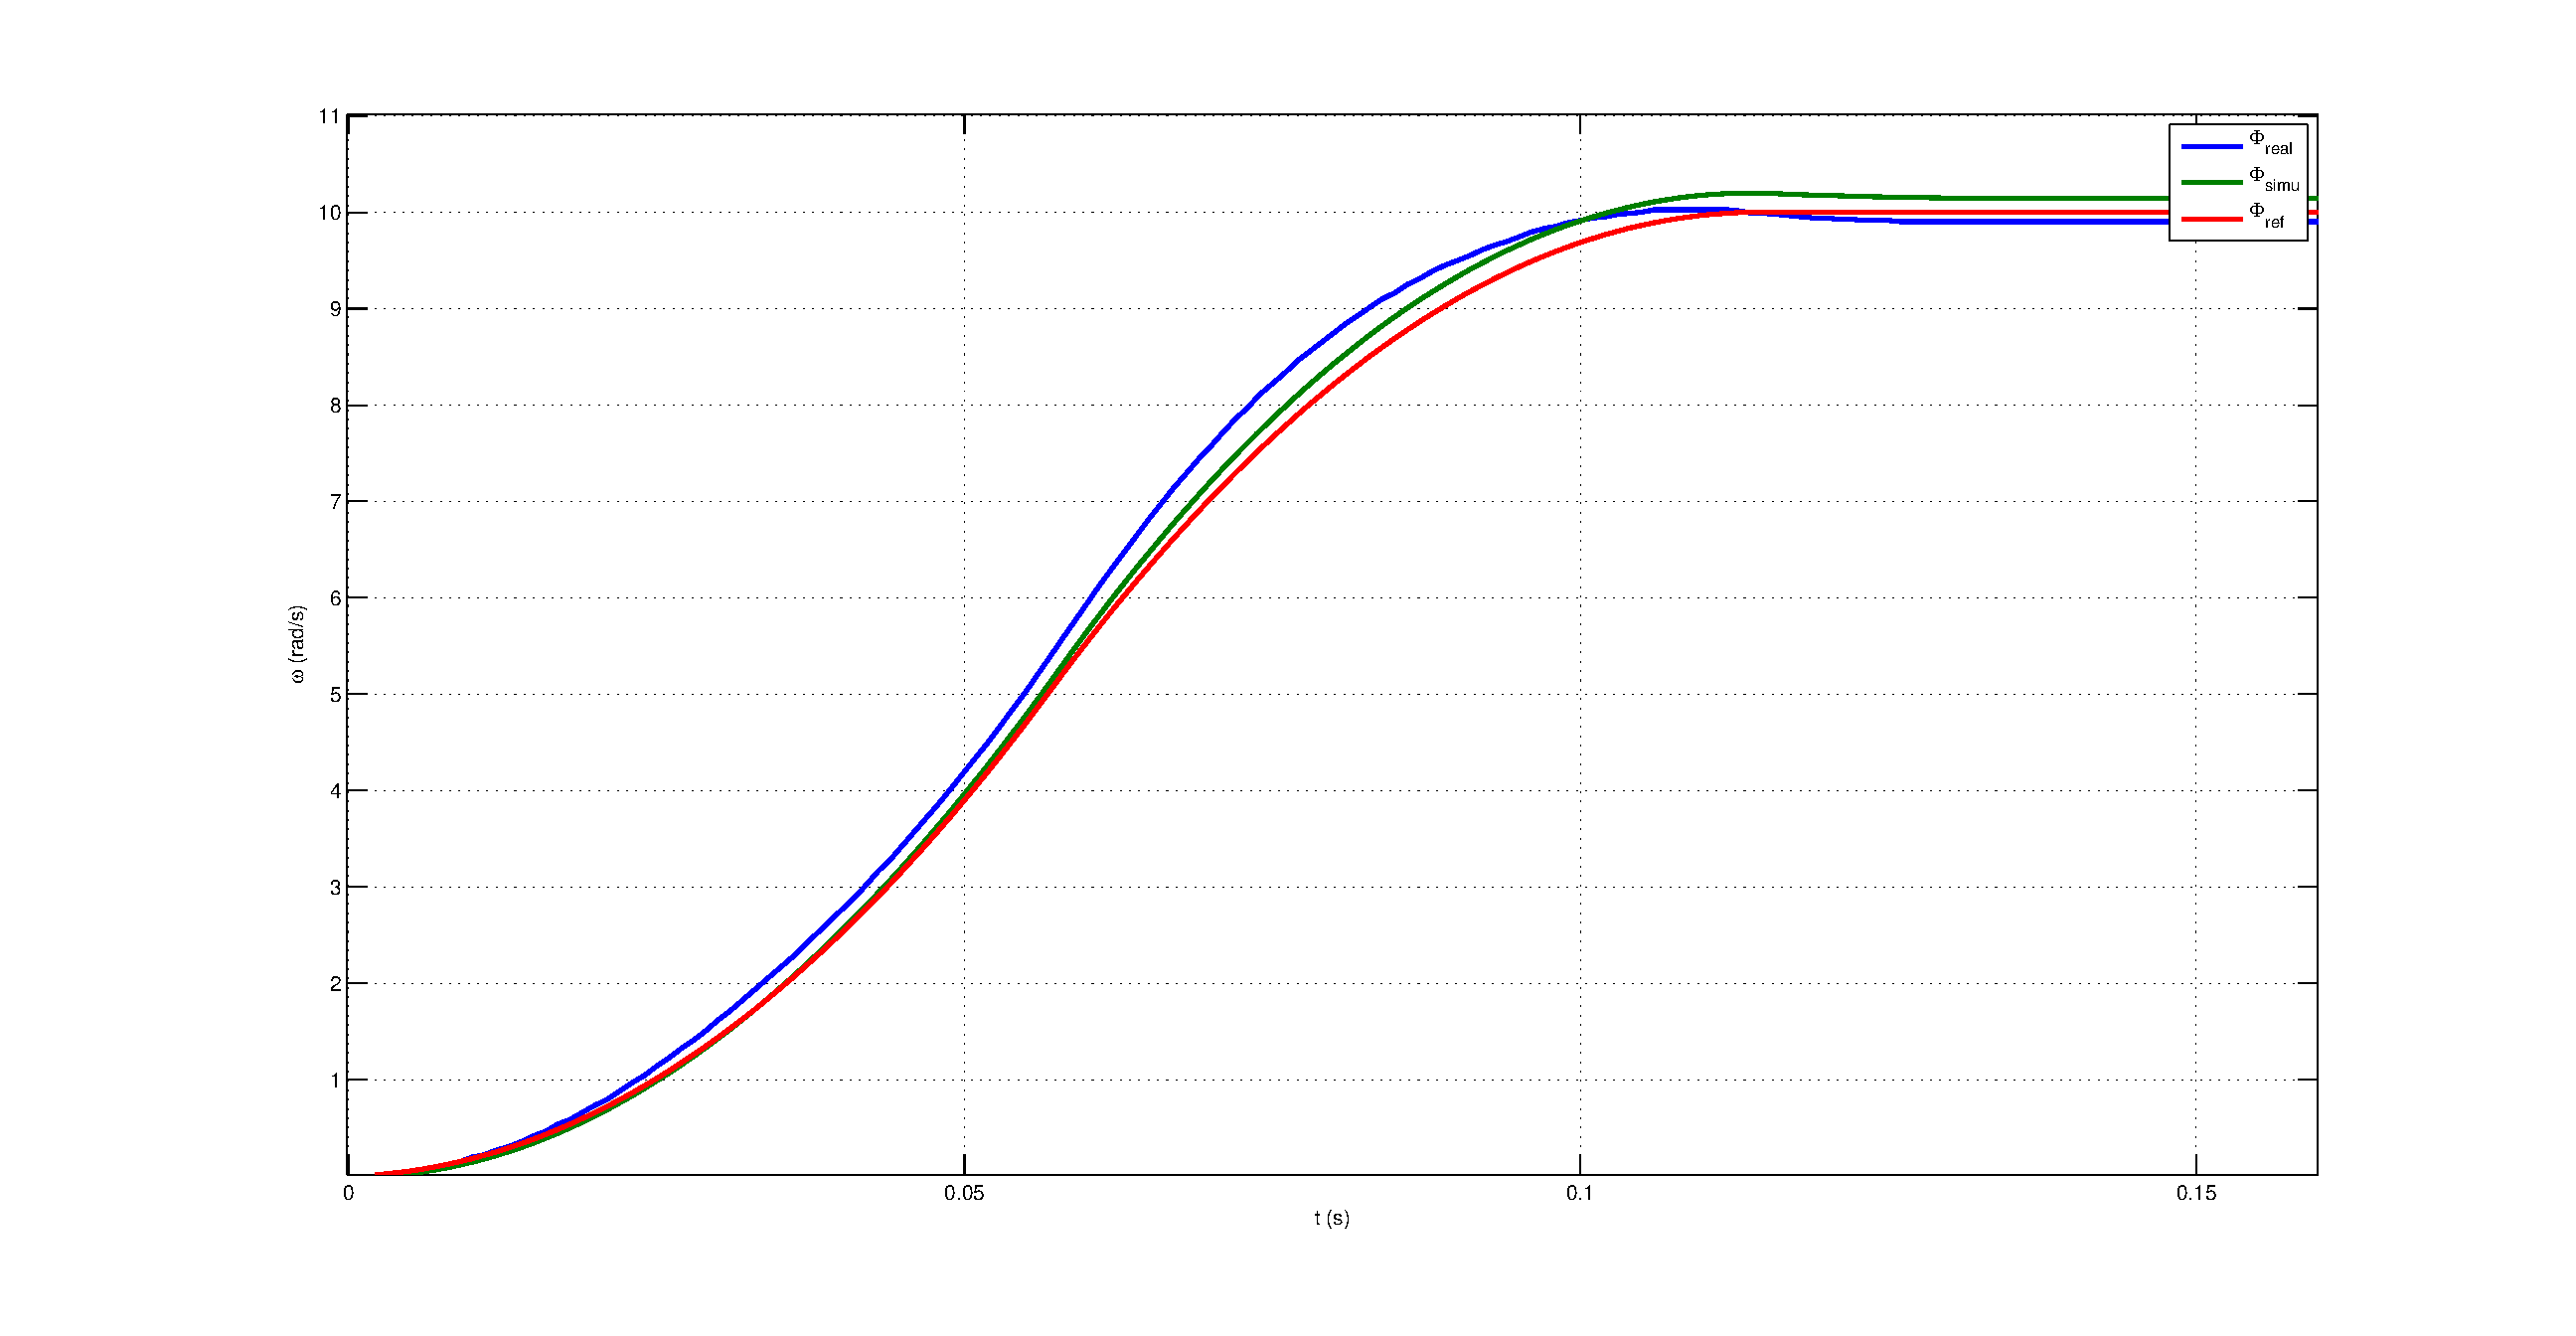
\includegraphics[width=\columnwidth]{fig/10rad.eps}
 \caption{$R_s = 10\text{[rad]}$}
 \end{subfigure}
 \begin{subfigure}[b]{\linewidth}
 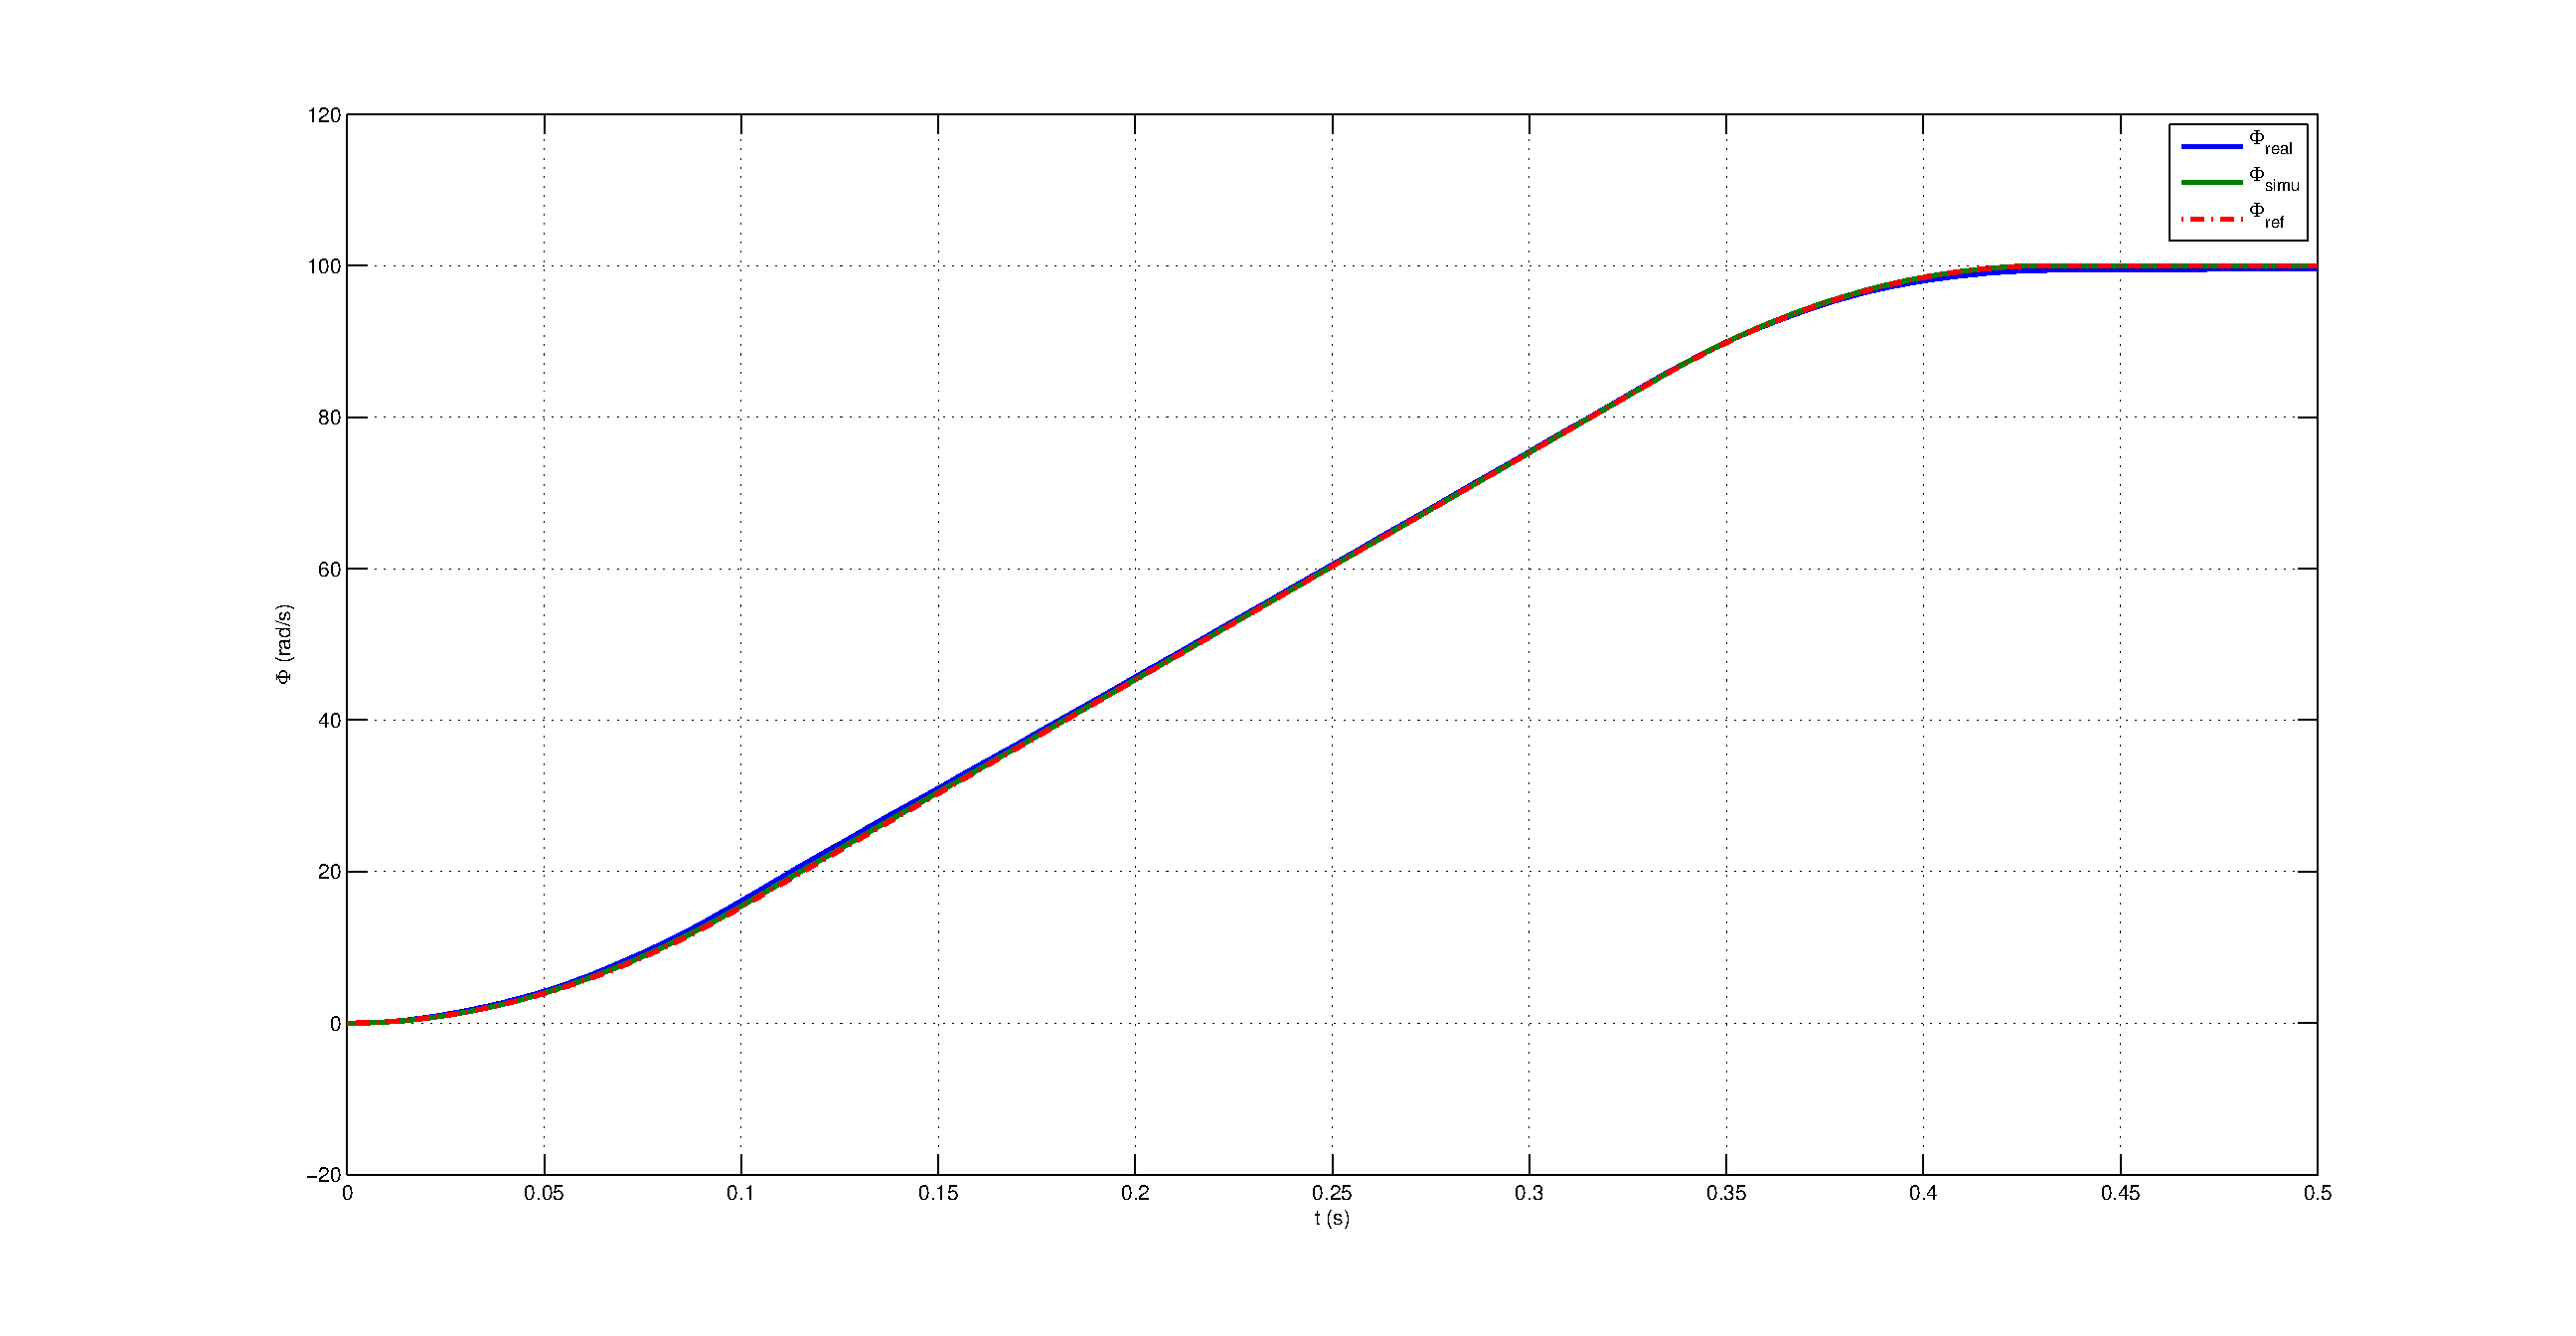
\includegraphics[width=\columnwidth]{fig/100rad.eps}
 \caption{$R_s = 100\text{[rad]}$}
 \end{subfigure}
 \caption{Simulation and real results \\ (blue) -- Real step response \\ (green) -- Simulated step response \\ (red) -- Reference}
 \label{realresults}
\end{figure}
